\section{Key defintions}

\begin{wrapfigure}{r}{0.40\textwidth}
    \centering
    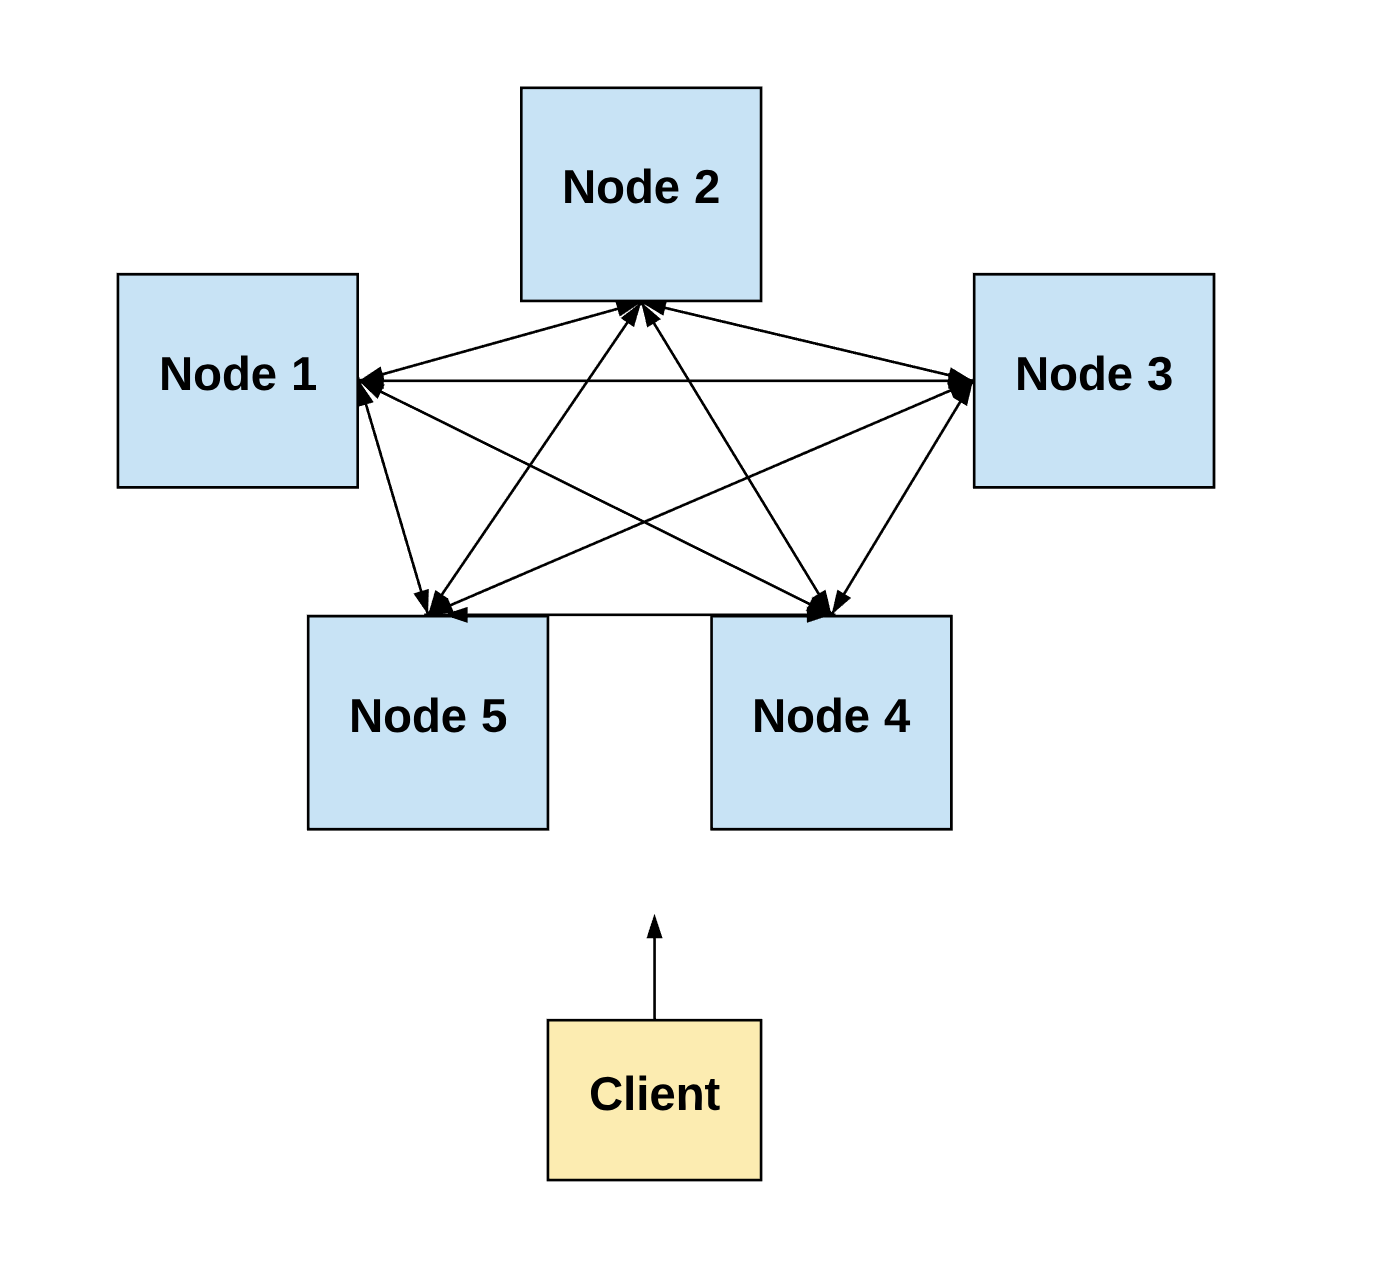
\includegraphics[width=0.40\textwidth]{time-synchrony-failures/key-definitions/assets/5-node-distributed-system.png}
    \caption{An example distributed system with 5 nodes. It may not be necessary that all nodes are connected directly to each other, but all nodes together present themeselves as a single unit to server client.}
    \label{fig:five-node-distributed-system}
\end{wrapfigure}

We begin by setting the stage up for problem at hand. In distributed systems, almost always, we are dealing with a distributed set of nodes that wants to present themselves as a single entity to the client. While earlier, this distribution of nodes was done in the efforts of increasing the uptime of the system (if one node dies, the other node can stay alive and service requests); in modern times with blockchain setting, the same is desirable for a different reason: decentralization (no single node or small set of nodes can disrupt the entire system).

For all further discussions, assume there to be $N$ different \textbf{nodes} in some distributed system $S$. We can then denote each node as $n_0, n_1, ..., n_{N-1}$. A client $C$ communicates with $S$ by communicating with one of the nodes in $S$, as such each node responds to $C$ as if being a spokesperson of $S$, i.e. it presents the services to the client according to the "global view" of the distributed system. Each such node $n_i \in N$ maintains a local \emph{append-only} data structure maintaining the history of "actions" / "transactions" it has seen since start of the protocol which should mimic closely the "global view" of the system. We can call it the "local view" of $n_i$. The content of messages can be arbitrary but are chosen from a message space $M$, all possible messages.

\subsection{Consistency and Liveness}

We begin our analysis of a distributed systems by describing what properties we intend to see from such systems. In very crude terms we want the following two properties:
\begin{itemize}
    \item \textbf{Bad things don't happen / consistency}: We want all nodes to agree on the common history, i.e. no two nodes have a conflict over which transaction happened first. This is especially significant if two transactions $t_1$ and $t_2$ both intend to consume a single resource, A $\verb|write(a, 20)|$ followed by $\verb|write(a, 40)|$ is not equivalent to $\verb|write(a, 40)|$ followed by $\verb|write(a, 20)|$.
    \item \textbf{Good things happen / liveness}: We want \emph{valid} transactions from users to be accepted by the system. No user should be left starving.
\end{itemize}

Of course, these are strong claims, and we need to quantify the amount of consisteny and liveness that we desire. Here are some quantifications for the same:

\begin{itemize}
    \item \textbf{Strong consistency vs Eventual consistency}: \index{Strong consistency} \index{Consistency} \index{Eventual Consistency} Strong consistency presents with some upper bound time guarantee $\delta$ after which it is assured that each node in the network will have the right view of some transaction, i.e. if a transaction $t$ was included at time $T$, then after some $T+\delta$ all nodes have a consistent view of the status of the transaction. Often, a weaker version \textbf{eventual consistency} is however more practically feasible though. Eventual consistency provides similar guarantee of global view of transactions, however without some finite time bound $\delta$. This can also be thought of as consistency where $\delta \to \infty$.
    \item \textbf{Strong liveness vs Eventual liveness}: \index{Strong liveness} \index{Liveness} \index{Eventual Liveness} Strong liveness presents with some upper bound time guarantee $\delta$ after which it is assured that client $C$'s transaction will be included in the \emph{append-only} history of $S$, i.e. if a transaction $t$ was presented by client $C$ at time $T$, then after some $T+\delta$, $S$ includes it. Often, a weaker version \textbf{eventual liveness} is however more practically feasible though. Eventual liveness provides similar guarantee of liveness, however without some finite time bound $\delta$. This can also be thought of as liveness where $\delta \to \infty$.
\end{itemize}

To elaborate on the above, let's take the following example:

A distributed system $S$ consists of 3 nodes $N = \{n_0, n_1, n_2\}$. The client $C$ can interact with any one of the three nodes in $N$. Assume the local ledgers of all three nodes are empty, as in:
$$
n_0: {\verb|local view| = [\phi], \verb|known unprocessed txs| = \{\}}
$$
$$
n_1: {\verb|local view| = [\phi], \verb|known unprocessed txs| = \{\}}
$$
$$
n_2: {\verb|local view| = [\phi], \verb|known unprocessed txs| = \{\}}
$$ 
Later, $C$ presents transaction $t$ to $n_2$, hence the state becomes:
$$
n_0: {\verb|local view| = [\phi], \verb|known unprocessed txs| = \{\}}
$$
$$
n_1: {\verb|local view| = [\phi], \verb|known unprocessed txs| = \{\}}
$$
$$
n_2: {\verb|local view| = [\phi], \verb|known unprocessed txs| = \{t\}}
$$ 

We want the final state of the system, if it is acting as a single unit to settle at the following configuration:
$$
n_0: {\verb|local view| = [t], \verb|known unprocessed txs| = \{\}}
$$
$$
n_1: {\verb|local view| = [t], \verb|known unprocessed txs| = \{\}}
$$
$$
n_2: {\verb|local view| = [t], \verb|known unprocessed txs| = \{\}}
$$

Here, the movement of $t$ from "known unprocessed txs" to the "local view" of all nodes in the system constitutes "liveness". However, this happens in stages. First, $n_2$ moves $t$ from "unprocessed" to "local view". Later, it ask all the other nodes to updates themselves with his local view. This aspect of other nodes updating their local view to match $n_2$'s local view constitutes "consistency".

\subsection{Node honesty}
\index{Node honesty}
\label{subsection:node-honesty}
In distributed systems, we generally deal with different kind of node faults. We call a node "faulty" when it deviates intentionally or unintentionally from the regular, online, honest participation in the network.

The following are the different kind of faults categorized:
\begin{itemize}
    \item \textbf{Crash fault}: \index{Crash fault} When some node $n_i$ behaves honestly from some origin time $t_0$ to some aribitrary time $t_c$, after which it crashes / goes offline. This can be further subdivided into nodes that present a \textbf{Fail-stop} \index{Fail Stop} failure and nodes that present a \textbf{True crash fault} \index{True crash fault}. Nodes that fail-stop halts, notifies everyone of its death and does not respond to any further messages. The nodes that experience true crash fault do not notify on the other hand. Evidently, true crash faults are harder to detect and manage as the rest of the network has to infer through indirect means the halt of the node.
    \item \textbf{Omission fault}: \index{Omission fault} Omission fault is when a node $n_i$ does not present required messages that it should have presented in an ideal setting to the rest of the network. This could be acknowledgements, votes or any other message. It is to be noted that omission of a message may be due to unreliability in the underlying network instead of a malice at the node's end.
    \item \textbf{Byzantine fault}: \index{Byzantine fault} Byzantine fault is where a node $n_i$ can behave arbitrarily, i.e. we can assume nothing about the node's behavior. Some of the actions exercised by such node could be: behaving like an honest node for some time range, behaving like a crashed node for some other time range, omitting messages, sending deceptive messages in hopes of disrupting the consensus. It should be noted however that we still assume the cryptography is not broken, as breaking that would mean in a system secured by public-key cryptography, the byzantine node can imitate any other node with no restrictions.
\end{itemize}

\subsection{Network Synchrony}

\subsection{Consensus}
The replication problem in distributed systems could be summarised as follows. Assume a node $n_i$ has a local view $v* \in V$ with $V$ being the set of all possible local views. A honest $n_i$ would intend to disseminate $v*$ to all the other nodes. 

\index{Consensus}
Consensus in distributed systems is defined as any algorithm $A$ that satisfies the following properties:
\begin{itemize}
    \item \textbf{Termination}: All non-faulty processes eventually decide on some value $v_i \in V$.
    \item \textbf{Agreement}: All non-faulty processes decide on the same value $v \in V$, i.e. $v_i = v \forall n_i \in N$.
    \item \textbf{Validity}: All non-faulty processes decide on a value $v*$.
\end{itemize}

It is important to understand that all the above properties are for "non-faulty" processes, a.k.a. only the honest processes. See \ref{subsection:node-honesty} for definition of node faults.

It is also worthwhile noting that aiming for any 2 out of the above 3 properties does not present us with any useful protocol. This can be argued as below:

If we only aim for \emph{termination and agreement}, all the nodes at each step may decide on some hardcoded value $v' \in V$.

If we only aim for \emph{agreement and validity}, all the nodes at each step will try to convince every other node to accept their value $v_i$ and never respond to other's messages. The consensus halts when all nodes are convinced. Unless all nodes started with the same value $v$, the consensus never halts.

If we only aim for \emph{validity and termination}, all the nodes at each step will decide on their own local $v_i$.

\subsection{Permissioning}

\subsection{Global Clock}

\subsection{Public Key Interchange Infrastructure}